% !TEX root = ../main.tex
\section{Data Analysis} \label{sec::dataanalysis}
    The first section on this chapter describes a C program developed by the author to perform the analysis in this thesis.
    Then, the second section talks about the Deep Inelastic Scattering (DIS) kinematics which define the cuts made to the data.
    The third section goes into detail about the approach to include sampling fraction to the analysis.
    Finally, the last section describes the simulations produced and the acceptance study made based on these.

    % !TEX root = ../main.tex
\subsection{\texttt{clas12-rge-analysis}} \label{ssec::clas12rgeanalysis}
    To perform the acceptance analysis reported in this thesis, the author developed an extensive C/C++ program running over the ROOT library.
    The purpose of this program is not only to do this analysis, but to be used in general in RG-E analysis.
    The program and its source are freely available under the GNU LGPLv3 license, and can be seen on GitHub at \hyperlink{https://github.com/bleaktwig/clas12-rge-analysis}{https://github.com/bleaktwig/clas12-rge-analysis}.
    Issues and pull requests are welcome, and are a crucial part to enable maintainability and collaborative development to the repository.

    After compiling the program via \texttt{make}, five executables are obtained in the \texttt{bin} directory.
    The following sections describe each.

    % !TEX root = ../main.tex
\subsubsection{\texttt{hipo2root}}
    CLAS12 reconstruction uses a custom data file named High-Performance Input Output (HIPO) format, developed by Gagik Gavalian \cite{chekanov2021}.
    The CLAS collaboration provides a set of tools to work with this format, allowing to read, write, and draw plots from HIPO files.
    Despite this, however, users at RG-E are much more familiar with the traditional ROOT files, and thus a conversion tool was developed.

    \texttt{hipo2root} filters through a HIPO file's data, and creates a ROOT file with pre-selected sections of storage, called banks.
    The selection of banks is based on data that is useful to RG-E analysis, and a user can easily add additional banks by editing the program's source files.
    The output of the executable is a ROOT file containing the selected banks as trees, a standard ROOT array-like variable.

    It's manual entry is:
    \begin{lstlisting}
Usage: hipo2root [-hfn:w:] infile
 * -h         : show this message and exit.
 * -f         : set this to true to process FMT::Tracks bank.
 * -n nevents : number of events.
 * -w workdir : location where output root files are to be stored. Default is root_io.
 * infile     : input HIPO file. Expected file format is <text>run_no.hipo.

Convert a file from hipo to root format. This program only conserves the banks that are useful for RG-E analysis, as specified in the `lib/bank_containers.h` file. It is important for the input hipo file to specify the run number at the end of the filename (`<text>run_no.hipo`), so that `hipo2root` can get the beam energy from the run number.

Since simulation files don't have a run number, we use a convention for specifying the beam energy. For this files, the filename should be `<text>999XXX.hipo`, where `XXX` is the beam energy used in the simulation in [0.1*GeV]. Currently, there are only 3 possible run numbers for simulations: 999106, 999110, and 999120. It is a pending task to improve this standard.
    \end{lstlisting}

    % !TEX root = ../main.tex
\subsubsection{\texttt{extract\_sf}}
    Some analysis from CLAS12 is needed to obtain the sampling fraction of the detector's calorimeters.
    This is done by the \texttt{extract\_sf} executable, which uses the particles' momenta and deposited energy.
    The exact methodology and results obtained are discussed in section \ref{ssec::sampling_fraction}.

    The manual entry of the program is:
    \begin{lstlisting}
Usage: extract_sf [-hfn:w:d:] infile
 * -h         : show this message and exit.
 * -n nevents : number of events
 * -w workdir : location where output root files are to be stored. Default is root_io.
 * -d datadir : location where sampling fraction files are located. Default is data.
 * infile     : input ROOT file. Expected file format: <text>run_no.root.

Obtain the EC sampling fraction from an input file. An alternative to using this program is filling the output file (by default stored in the `data` directory) with the data obtained from [CCDB](https://clasweb.jlab.org/cgi-bin/ccdb/versions?table=/calibration/eb/electron_sf). The function used to fit the data is

[0]*Gaus(x,[1],[2]) + [3]*x*x + [4]*x + [5]

where [0] is the amplitude of the Gaussian, [1] and [2] its mean and sigma, and [3], [4], and [5] the p0, p1, and p2 used to fit the background.

The output of the program is the `sf_params_<run_no>.txt`, which contains a table with the sampling fractions and their errors. The table is formatted like the one at CCDB, as in

         | sf0    sf1    sf2    sf3    sfs1   sfs2   sfs3   sfs4
---------+--------------------------------------------------------
sector 1 | %11.8f %11.8f %11.8f %11.8f %11.8f %11.8f %11.8f %11.8f
sector 2 | %11.8f %11.8f %11.8f %11.8f %11.8f %11.8f %11.8f %11.8f
sector 3 | %11.8f %11.8f %11.8f %11.8f %11.8f %11.8f %11.8f %11.8f
sector 4 | %11.8f %11.8f %11.8f %11.8f %11.8f %11.8f %11.8f %11.8f
sector 5 | %11.8f %11.8f %11.8f %11.8f %11.8f %11.8f %11.8f %11.8f
sector 6 | %11.8f %11.8f %11.8f %11.8f %11.8f %11.8f %11.8f %11.8f
    \end{lstlisting}

    % !TEX root = ../main.tex
\subsubsection{\texttt{acc\_corr}}
\label{sssec::acc_corr}
    The \texttt{acc\_corr} executable is used to count the number of thrown and simulated events from two different ROOT files.
    Based on the program's input, it separates the data into appropriate 5-dimensional bins, counts the entries for all available particles in the generated file, and exports the results into a text file.
    The results and plots presented in section \ref{ssec::acceptance_correction} were generated using the data obtained from this program.

    The manual entry of the program is:
    \begin{lstlisting}
Usage: acc_corr [-hq:n:z:p:f:g:s:d:FD]
 * -h         : show this message and exit.
 * -q ...     : Q2 bins.
 * -n ...     : nu bins.
 * -z ...     : z_h bins.
 * -p ...     : Pt2 bins.
 * -f ...     : phi_PQ bins (in degrees).
 * -g genfile : generated events ROOT file.
 * -s simfile : simulated events ROOT file.
 * -d datadir : location where sampling fraction files are found.
                Default is data.
 * -F         : flag to tell program to use FMT data instead of DC data
                from the simulation file.
 * -D         : flag to tell program that generated events are in
                degrees instead of radians.

Get the 5-dimensional acceptance correction factors for *Q2*, *nu*, *z_h*, *Pt2*, and *phi_PQ*. For each optional argument, an array of doubles is expected. The first double will be the lower limit of the leftmost bin, the final double will be the upper limit of the rightmost bin, and all doubles between them will be the separators between each bin.

The output will be written to the `acc_corr.txt` file, by default in the `data` directory, which is formatted to make it easy to read by the `draw_plots` program:
* First line contains five integers; the size of each of the five binnings.
* The next five lines are each of the binning schemes, in order *Q2*, *nu*, *z_h*, *Pt2*, and *phi_PQ*.
* The following line contains one integer which is the size of the list of PIDs, followed by a line containing each of these PIDs.
* Finally, a number of lines equal to the number of PIDs follows. Each line contains a list of the bins, ordered as `[Q2][nu][z_h][Pt2][phi_PQ]`.
    \end{lstlisting}

    % !TEX root = ../main.tex
\subsubsection{\texttt{make\_ntuples}}
    This executable runs over one or more files generated by \texttt{hipo2root} and saves a ROOT file containing a set of ntuples of physical interest.
    In addition, based on the requirements for this thesis' analysis, the executable generates two sets of ntuples.
    Both sets contain the same ntuple format, but the former uses only DC tracking data while the latter uses DC and FMT tracking data.
    
    For each event, the program executes the following algorithm:
    
    \begin{enumerate}
        \item
            First, the TOF of the trigger electron is to be found.
            The trigger electron's hits in the FD scintillators and FD calorimeters are listed in order of priority.
            This priority comes from the precision of each detector's TOF measurement.
            In order of precision, the detectors list is FTOF panel-1b (FTOF1B), FTOF panel-1a (FTOF1A), FTOF panel-2 (FTOF2), Pre-shower Calorimeter (PCAL), ECIN, ECOU, as described in section \ref{sssec::forwarddetector}.
            Then, the list of hits is simply iterated over, extracting the TOF from the earliest hit of the most precise layer available.
    
        \item
            Then, for each track available two particle objects is instantiated.
            This object contains the particle's relevant data: it's vertex position, vertex momentum, charge, beta, and the CLAS12 sector where it passed through.
            The first object corresponds to tracking data obtained by DC, while the second to DC and FMT.
            The particle's PID will be assigned later in the process.
            
        \item
            The particle's deposited energy in the calorimeters is computed and stored.
            This simply means adding the energy deposited by all the hits associated to the particle's track, for each calorimeter.
        
        \item
            The particle's number of produced photoelectrons in HTCC and LTCC is counted.
            Additionally, its TOF is computed, following the same procedure as the one for the trigger electron's TOF.
        
        \item
            The particle's PID is assigned.
            The process is very similar to the assignment of PID in reconstruction, which is described in section \ref{sssec::offlinereconstruction}.
            However, this PID is not directly used, to allow the user to modify the parameters and define new criteria to assign PID.

            While this process gives almost always the same result as reconstruction, there is a slight error in the PID assignment.
            This error is expressed in table \ref{tab::mpid}.
            As can be seen on the table, some kaons and protons are misidentified as pions, but not to a large degree.
            Apart from that, all identification is ideal.
            
            \begin{table}
                \caption{Particle identification matrix for the FD.
                The rows show the PID assigned by reconstruction while the columns the one assigned by the \texttt{make\_ntuples} program.
                The diagonal elements are correctly identified, while the off-diagonal elements are misidentified.}

                \begin{center}
                    \begin{tabularx}{240pt}{X|llllll}
                        \cline{2-7}
                                 & $e$      & $\pi$ & $K$  & $p$  & $n$  & $\gamma$ \\
                        \hline
                        $e$      & 1.00     &       &      &      &      &          \\
                        $\pi$    &          & 1.00  & 0.09 & 0.02 &      &          \\
                        $K$      &          &       & 0.91 &      &      &          \\
                        $p$      &          &       &      & 0.98 &      &          \\
                        $n$      &          &       &      &      & 1.00 &          \\
                        $\gamma$ &          &       &      &      &      & 1.00     \\
                        \hline
                    \end{tabularx}
                \end{center}
                \label{tab::mpid}
            \end{table}

        \item
            Finally, two \texttt{ntuples} objects are created: One from the particle generated from DC tracking data and another for the one from DC plus FMT data.
            These are saved in an output file, which can be used directly for analysis, or processed by the \texttt{draw\_plots} program from the next section.
    \end{enumerate}

    The manual entry of the program is:
    \begin{lstlisting}
Usage: make_ntuples [-hDn:w:d:] infile
 * -h         : show this message and exit.
 * -D         : activate debug mode.
 * -n nevents : number of events.
 * -f         : set this to true to process FMT::Tracks bank.
 * -w workdir : location where output root files are to be stored. Default is root_io.
 * -d datadir : location where sampling fraction files are located. Default is data.
 * infile     : input ROOT file. Expected file format: <text>run_no.root`.

Generate ntuples relevant to SIDIS analysis based on the reconstructed variables from CLAS12 data. The output of the program is the `ntuples_<run_no>.root` file, which contains all relevant ntuples for RG-E analysis. This file can be studied directly in root or through the `draw_plots` program.
    \end{lstlisting}
    % !TEX root = ../main.tex
\subsubsection{\texttt{draw\_plots}}
    This executable is included so that the user doesn't have to re-write similar code regularly to obtain plots.
    Operating \texttt{draw\_plots} is fairly simple: after running the program, the user must answer a set of question to define the various attributes related to the plots.
    This includes cuts and corrections to apply, binning setup, and, naturally, the variables in the plots.
    Unless otherwise specified, the plots included in section \ref{sec::resultsandconclusions} were produced using this executable.

    The executable's manual entry is:
    \begin{lstlisting}
Usage: draw_plots [-hp:cn:o:a:w:] infile
 * -h          : show this message and exit.
 * -p pid      : skip particle selection and draw plots for pid.
 * -c          : apply all cuts (general, geometry, and DIS) instead of
                 asking which ones to apply while running.
 * -n nentries : number of entries to process.
 * -o outfile  : output file name. Default is plots_<run_no>.root.
 * -a accfile  : apply acceptance correction using acc_filename.
 * -A          : get acceptance correction plots without applying acceptance
                 correction. Requires -a to be set.
 * -w workdir  : location where output root files are to be stored. Default
                 is root_io.
 * infile      : input file produced by make_ntuples.\n

Draw plots from a ROOT file built from `make_ntuples`. File should be named `<text>run_no.root`. This tool is built for those who don't enjoy using root too much, and should be able to get most basic plots needed in SIDIS analysis.
    \end{lstlisting}


    % !TEX root = ../main.tex
\subsection{Cuts} \label{ssec::cuts}
    Three types of cuts are applied to particles to increase their value for the analysis provided in this work:
    \begin{itemize}
        \item
            General cuts, which exclude badly reconstructed particles.
        \item
            Geometry cuts, which limit the region from where reconstruction data is useful for this analysis.
        \item
            DIS cuts, which limit the region of analysis to that of DIS.
    \end{itemize}

    Only two cuts are considered ``general'' for this analysis.
    The first one simply filters out particles with PID $0$ or $45$.
    These PIDs are used in CLAS12 reconstruction to denote particles whose PID couldn't be successfully identified.
    Then, the second filters out particles whose tracking is not very precise, and is defined as
    \begin{equation*}
        \frac{\chi^2}{\text{NDF}} < 15,
    \end{equation*}
    where $\chi^2$ is the final result from the $\chi^2$-test used to guide the Kalman filter fit in the tracking algorithm, as described in \ref{sssec::offlinereconstruction}, and NDF is the number of degrees of freedom of this same fit.

    \begin{figure}[b!]
        \centering\frame{
        \includegraphics[width=\textwidth]{13dataanalysis/img/20q2_vs_nu.pdf}}
        \caption[$Q^2$ vs $\nu$ comparison]{$Q^2$ vs $\nu$ before and after applying the $Q^2 > 1$ and $W^2 > 4$ cuts.}
        \label{fig::q2vsnu}
    \end{figure}

    The geometry cuts also include two cuts, both working to constrain the vertex of the reconstructed particle to the beamline.
    The first one secures us that the vertex comes from the beamline, and is given by
    \begin{equation*}
        \sqrt{v_x^2 + v_y^2} < 4 \text{ cm},
    \end{equation*}
    where $v_x$ and $v_y$ are the $x$ and $y$ coordinates of the vertex position.
    The second one ensures that the hit comes from the target, and is
    \begin{equation*}
        -40 \text{ cm} < v_z < 40 \text{ cm},
    \end{equation*}
    where $v_z$ is the $z$ coordinate of the vertex position.
    This cut is defined from the shape of the RG-F target.

    Finally, the DIS cuts are cuts made on the scattered electron to limit the phase space to that of DIS.
    All particles in an event are ignored if the trigger electron doesn't pass these cuts.

    First, a cut is applied on the invariant mass of the virtual photon, $Q^2$, which is
    \begin{equation*}
        Q^2 > 1 \text{ GeV}^2,
    \end{equation*}
    ensuring that we are in the domain of DIS.

    Then, a cut is made on the squared mass of the hadronic final state, $W^2$, given by
    \begin{equation*}
        W^2 > 4,
    \end{equation*}
    where $W^2$ is defined by
    \begin{equation*}
        W^2 = M^2 + 2M\nu - Q^2,
    \end{equation*}
    and $M$ is the nucleon mass, and $\nu$ is the energy fraction of the virtual photon.
    This cut is applied to exclude nucleon resonances.

    The effect of these cuts on $Q^2$ and $\nu$ can be seen on plot \ref{fig::q2vsnu}.

    % !TEX root = ../main.tex
    \begin{figure}[b!]
        \centering\frame{
        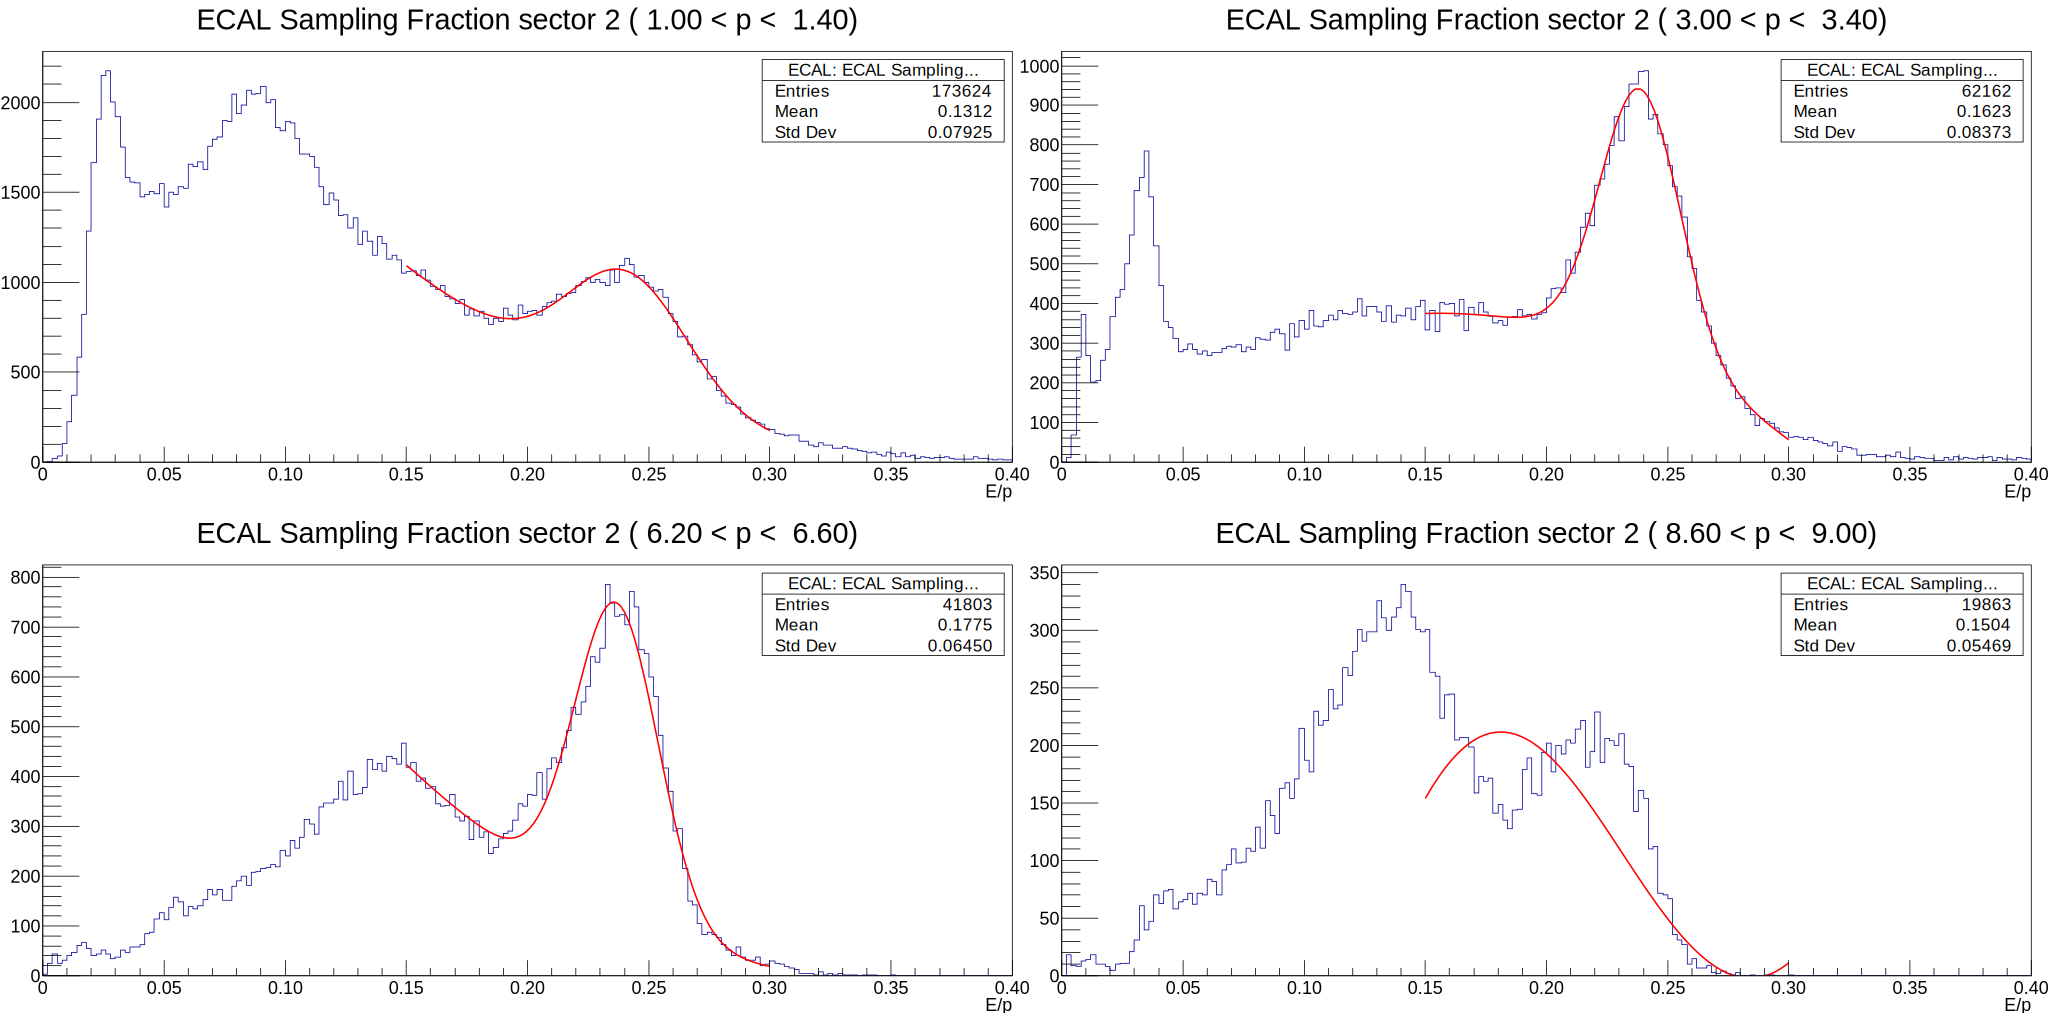
\includegraphics[width=\textwidth]{13dataanalysis/img/30sf_1d_plots.pdf}}
        \caption[Calorimeters $E/p$ plots]{Four $E/p$ plots describing the sum of the deposited energy per particle on all calorimeters (PCAL, ECIN, and ECOU). The particles' momentum is obtained from tracking and the event builder. As can be seen in the northwest and the southeast plots, the corner bins -- $1.00$ to $1.40$ and $8.60$ to $9.00 [\text{GeV}]$ respectively -- are not very reliable.}
        \label{fig::sf_1d}
    \end{figure}

\subsection{Sampling Fraction} \label{ssec::sampling_fraction}
    The energy deposited by electrons in the active area of the calorimeters is a fraction of their total energy $E_\text{tot}$.
    This value is proportional to their momentum $P$ for energies above a few hundred MeV.
    Heavier particles, due to their reduced penetration capabilities, tend to lose an amount of energy independent from their momentum.
    An electron sampling fraction measures the amount of energy lost depending on the momentum of a particle.
    This allows both the measurement of the electron's energy and the differentiation of electrons from other particles \cite{wigmans2000}.

    % Explain how the executable extracts the sampling fraction.
        % Show plot with curve of means!
    To obtain the sampling fraction, the hits of each calorimeter by itself (PCAL, ECIN, and ECOU) are separated in arrays, with an additional array containing the union of the three others.
    Then, these arrays of hits are separated into 20 momentum bins.
    Each bin has a size of $0.4 [\text{GeV}]$, starting at $1.0 [\text{GeV}]$ and ending at $9.0 [\text{GeV}]$.

    1-dimensional histograms are then drawn from the data in these arrays, measuring deposited energy divided by vertex momentum ($E/p$).
    A Gaussian fit plus quadratic background is then applied, as described by the following function:
    \begin{equation*}
        f(x) = p_0 g(x, \mu, \sigma) + p_1 x^2 + p_2 x + p_3, \hspace{12pt}
        \text{where} \hspace{4pt}
        g(x, \mu, \sigma) = \frac{1}{\sigma \sqrt{2\mu}} \exp \left(-\frac{1}{2} \frac{(x - \mu)^2}{\sigma^2}\right),
    \end{equation*}
    where $\mu$ and $\sigma$ are the mean and standard deviation of the distribution, respectively.
    Since the expected range of deposited energy $E/p$ expected for electrons is between $0.15$ to $0.30$ from theory, the fit is limited to that range.

    Examples of these plots are given in figure \ref{fig::sf_1d}.
    As can be seen in the figure, not enough electrons are seen in extreme momentum ranges, like from $1$ to $1.4$ GeV or from $8.6$ to $9$ GeV.
    Due to this, the sampling fraction fit described later only considers data in the range from $1.4$ to $8.6$ GeV.

    The mean of each of these fits is then extracted to be used as data points for a sampling fraction fit.
    A polynomial fit is used, since it follows well the shape of these points, and is what's used in the reconstruction software.
    The fit described by
    \begin{equation*}
        f(x) = p_0 \cdot \left(p_1 + \frac{p_2}{x} + \frac{p_3}{x^2}\right),
    \end{equation*}
    The $E/p$ distribution vs $p$ is shown in figure \ref{fig::sf_2d} along with this fit.

    \begin{figure}[t!]
        \centering\frame{
        \includegraphics[width=\textwidth]{13dataanalysis/img/30sf_2d_plot.pdf}}
        \caption[Calorimeters $p vs E/p$ plots]{A 2d plot showing momentum $p$ vs deposited energy divided by momentum $E/p$. The particle's deposited energy on all calorimeters is measured. Its momentum is obtained from tracking and the event builder. The fit follows the deposited energy of electrons to find their sampling fraction.}
        \label{fig::sf_2d}
    \end{figure}

    Finally, the parameters of the fit are stored in plain text files, following the convention in the CCDB.
    The parameters obtained can later be used to perform particle identification for electrons and photons.
    In addition, they are used to obtain the energy of electrons and photons since, as mentioned before, not all of it is deposited in the calorimeters.

    % !TEX root = ../main.tex
\subsection{Acceptance Correction} \label{ssec::acceptance_correction}
% --+ What is acceptance +------------------------------------------------------
    When discussing radiation detection, it is common to describe two types of efficiency: absolute efficiency and intrinsic detection efficiency.
    The former is defined as the fraction of events emitted by the source which is actually registered by the detector, or
    \begin{equation*}
        \xi_\text{tot} = \frac{\text{events registered}}{\text{events emitted by source}}.
    \end{equation*}
    This is a function of the detector geometry and the probability of an interaction in the detector.
    Total efficiency is also known as detector acceptance.

    Then, this total efficiency can be factored into two parts: the intrinsic efficiency, $\xi_{\text{int}}$, and the geometric efficiency, $\xi_{\text{geom}}$.
    The total efficiency is then given by
    \begin{equation*}
        \xi_\text{tot} = \xi_\text{int} \cdot \xi_\text{geom}.
    \end{equation*}

    The intrinsic efficiency is that fraction of events actually hitting the detector which is registered
    \begin{equation*}
        \xi_\text{int} = \frac{\text{events registered}}{\text{events impinging on detector}}.
    \end{equation*}
    This probability depends on the interaction cross sections of the incident radiation on the detector medium.
    The intrinsic efficiency is thus a function of the type of radiation, its energy and the detector material \cite{leo1987}.

% --+ Acceptance correction through generation + simulation +-------------------
    Acceptance correction is the process of correcting for the total efficiency of the detector.
    To obtain an estimation of this detector efficiency, we can compare the total generated events $N_\text{thrown}$ with the accepted events in a simulation of the detector $N_\text{simul}$, such that
    \begin{equation*}
        \tilde\xi_\text{tot} = \frac{N_\text{simul}}{N_\text{thrown}}.
    \end{equation*}
    This quantity is naturally dependent on the quality of the event generator and simulation programs.

% --+ Chosen bins +-------------------------------------------------------------
    Acceptance varies along the phase space of the kinematical variables.
    Thus, to make the correction accurate, the ratio must be separated into five-dimensional bins.
    These correspond to the five studied variables, $Q^2$, $\nu$, $z_h$, $p_T^2$, and $\phi_{PQ}$.
    For simplicity in analysis, all bins for a variable are of the same size, such that the results are easy to interpret.
    % The bins are designed such that there is a similar number of entries in each, with the additional requirement that the histogram curve is as linear as possible.
    \begin{itemize}
        \item
            $Q^2 = 4E_bE'\sin^2(\theta_C/2)$ is the 4-momentum transferred by the lepton probe in the lab frame, where $E_b$ is the beam energy, $E'$ is the scattered electron's energy, and $\theta_C$ is the polar angle of the scattered electron.
            The chosen bin edges are $1$, $2$, $3$, $4$, $5$, $6$, $7$, $8$, $9$, $10$, $11.0$ $\text{GeV}^2$.
        \item
            $\nu = E_v - E'$ is the energy transferred by the lepton probe in the lab frame.
            The chosen bin edges are $2$, $3$, $4$, $5$, $6$, $7$, $8$, $9$, and $10$ $\text{GeV}$.
        \item
            $z_h = E_h/\nu$ is the virtual photon energy fraction carried by the measured hadron, with $E_h$ being this hadron's energy.
            The chosen bin edges are $0$, $0.1$, $0.2$, $0.3$, $0.4$, $0.5$, $0.6$, $0.7$, $0.8$, $0.9$, and $1$.
        \item
            $p_T^2$ is the hadron's transverse momentum measured with respect to the virtual photon direction.
            The chosen bin edges are $0$, $0.2$, $0.4$, $0.6$, $0.8$, $1$, $1.2$, $1.4$, $1.6$, $1.8$, and $2$ $\text{GeV}^2$.
        \item
            $\phi_{PQ}$ is the angle between the leptonic plane -- the plane where the paths of the initial and scattered electrons lie -- and the hadronic plane, which contains the virtual photon and the measured hadron.
            The chosen bin edges are $-180$, $-140$, $-100$, $-60$, $-20$, $20$, $60$, $100$, $140$, and $180$ degrees.
    \end{itemize}

    Plots for each of the variables described with vertical lines showing the bins can be seen in the plots to the left of figure \ref{fig::acc_corr}.
    The data used to obtain these plots is from RG-F run number $\mathbf{012933}$, which contains a total of $23,844,549$ reconstructed events to work with.
    % TODO. What to do about this? Just use less bins?

    To compute the acceptance, 10 million events were generated in deep inelastic kinematics using LEPTO, a Monte Carlo generator for deep inelastic lepton-nucleon scattering \cite{ingelman1997}.
    Then, the events were simulated in the RG-F experiments conditions in CLAS12 by using \texttt{gemc}, with a torus field polarity of $-1$ and solenoid field polarity of $-0.745033$.
    \texttt{gemc} is the standard tool used for simulating CLAS12 events \cite{ungaro2020gemc}.
    Finally, they were reconstructed using \texttt{coatjava}, the standard tool for CLAS12 event offline reconstruction \cite{ziegler2020}.
    A description of the last can be read in section \ref{sssec::offlinereconstruction}.
    The results of the acceptance correction process are discussed in section \ref{ssec::acceptancecorrectionresults}.

